\section{Finite Difference Method}

The finite difference method (FDM) is a numerical method used to find an approximate 
solution to differential equations. It works by creating a discrete approximation 
of the derivative and using this approximation to write the differential equation 
as a system of linear equations.

There are different versions of the finite difference method.
\begin{itemize}
	\item Forward difference, $\Delta_hf(x) = f(x+h) - f(x)$
	\item Backward difference, $\nabla_hf(x) = f(x) - f(x - h)$
	\item Central difference, $\delta_hf(x) = f(x + \frac{1}{2}h) - f(x - \frac{1}{2}h)$
\end{itemize}

It is easy to see the connection of the forward difference and the definition of 
the derivative.

$$f'(x) = \lim_{h \to 0} \frac{f(x+h) - f(x)}{h}$$

We give $h$ a fixed, non-zero, value instead of having $h$ approach 0. Therefore 
the forward difference divided by $h$ approximates the derivative when $h$ is small.

$$f'(x) \approx \frac{f(x+h) - f(x)}{h}$$

TODO: Write about the error in the approximation

The second order derivative can be approximated by applying the finite difference 
approximation to each term in the already derived expression for the approximation. 
For the central difference approximation another central difference approximation 
is applied to $f'(x + \frac{1}{2}h)$ and $f'(x - \frac{1}{2}h)$. This results in 
the following second order central difference approximation:

$$f''(x) \approx \frac{\delta_h^2f(x)}{h^2} = \frac{f(x+h) - 2f(x) + f(x-h)}{h^2}$$

When applied to higher dimensions, it is necessary to choose a value for h in 
each dimension. However we can simplify the resulting equation by choosing the same h. 
In three dimensions the approximation looks like this:

$$(\pTwo{x} + \pTwo{y} + \pTwo{z}) f (x, y, z) = \frac{\partial^2 f(x, y, z)}{\partial^2 x} 
+ \frac{\partial^2 f(x, y, z)}{\partial^2 y} + \frac{\partial^2 f(x, y, z)}{\partial^2 z}$$

$$\frac{\partial^2 f(x, y, z)}{\partial^2 x} \approx \frac{f(x+h, y, z) - 2f(x, y, z) + f(x-h, y, z)}{h^2}$$

$$\frac{\partial^2 f(x, y, z)}{\partial^2 y} \approx \frac{f(x, y+h, z) - 2f(x, y, z) + f(x, y-h, z)}{h^2}$$

$$\frac{\partial^2 f(x, y, z)}{\partial^2 z} \approx \frac{f(x, y, z+h) - 2f(x, y, z) + f(x, y, z-h)}{h^2}$$

This is also known as the 7-point stencil as illustrated in figure \ref{fig:7ps}.

\begin{figure}[ht]
	\center
	
\includegraphics[width=0.5\textwidth]{images/7_point_stencil}
	\caption{7-point stencil}
	\label{fig:7ps}
\end{figure}

\subsection{Discrete Poisson Equation}

To apply the finite difference method to the Poisson equation with Dirichlet 
boundary conditions, problem domain is sampled in a finite number of points. 
The distance between the sample points, $h$, is the same as the fixed $h$ in the finite
differences method. Lets consider the two-dimensional Poisson equation $\nabla^2
u(x, y) = f(x, y)$. We use the central difference approximation to sample
$\nabla^2 u(x, y)$ at $n+1$ points in the $x$ direction and $n+1$ points in $y$
direction. We assume the dimensions of the domain goes from $0$ to $1$. The discretized 
grid is illustrated in figure \ref{fig:discgrid}.

\begin{figure}[ht]
	\center
	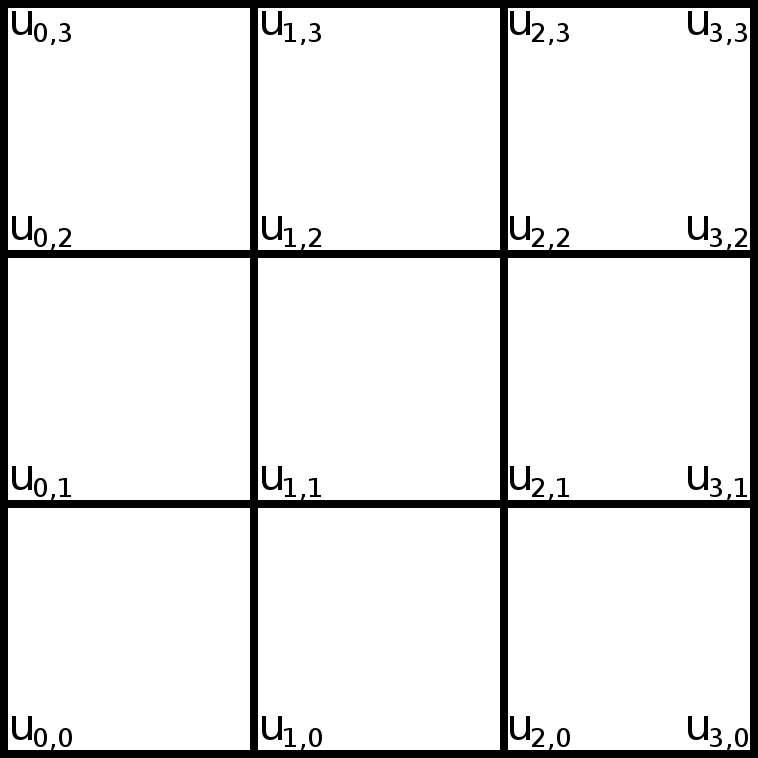
\includegraphics[width=0.6\textwidth]{images/2d_poisson_ex}
	\caption{Discretized grid with $n = 3$}
	\label{fig:discgrid}
\end{figure}

This gives $(n-1)^2$ internal points and the remaining points are boundary
points that have their values specified by the boundary conditions. The total
number of unknowns are therefore $N = (n-1)^2$.

$$h = \frac{1}{n}$$
$$x_i = ih, ~~~~ i = 0, 1, \dots, n$$
$$y_j = jh, ~~~~ j = 0, 1, \dots, n$$

We then denote the approximation of the value of $u(x_i, y_j)$ by $u_{i,j}$ and 
$f(x_i, y_j)$ by $f_{i,j}$

$$ (\nabla^2 u)_{ij} \approx \frac{u_{i+1,j} + u_{i,j+1} - 4u_{i,j} + u_{i-1,j} + u_{i,j-1}}{h^2} = f_{i,j} $$
$$ u_{i+1,j} + u_{i,j+1} - 4u_{i,j} + u_{i-1,j} + u_{i,j-1} = h^2 f_{i,j} $$

This creates a system of linear equations, which we want to write on matrix form.

$$Ax = b$$

To create this linear system we have to create a global order for the
internal nodes to create the $x$ vector of unknowns. We use the natural
order, which means that we list the nodes along the $x$ direction first.

$$x_k = u_{i,j}, ~ k = (i-1) + (n-1) \cdot (j-1), ~ i, j = 1, 2, \dots, n-1$$

We can then assemble the matrix $A$.

$$
A = \begin{bmatrix}
 B & I & 0 & \cdots & 0 \\
 I & B & I &   & \vdots \\
 \vdots &   & \ddots &   & \vdots \\
 \vdots &   &   & \ddots & \vdots \\
 0 & \cdots & \cdots & I & B 
\end{bmatrix}
~~
B = \begin{bmatrix}
-4 & 1 & 0 & \cdots & 0 \\
 1 &-4 & 1 &   & \vdots \\
 \vdots &   & \ddots &   & \vdots \\
 \vdots &   &   & \ddots & \vdots \\
 0 & \cdots & \cdots & 1 &-4 
\end{bmatrix}
$$

$A$ is a $N \times N$ matrix, $B$ is a $(n-1) \times (n-1)$ matrix and $I$ is the identity matrix.

The vector $b$ is assembled from $h^2$, the function $f$, and the Dirichlet border conditions. 

$$ b_k = h^2 \cdot f_{i,j} - u_{?} $$

TODO: how is $b$ made
